\documentclass{article}
\usepackage{graphicx}

\title{Tugas Besar Cara Membuat Aplikasi "Data Hasil Pertanian"}
\author{Murnia Lestari D4 Teknik Informatika 2C} 
\date{18 December 2019}

\begin{document}

\maketitle

\section{Langkah-langkah Membuat Aplikasi}
\begin{enumerate}
    \item Install oracle apex atau kamu juga dapat membuka oracle apex di browser.
    \par Jika kamu menggunakan oracle apex yang online ,maka terlebih dahulu kamu harus menginstall oracle apex lalu ikuti langkah-langkah penginstalan dengan benar.Sehingga aplikasi dapat digunakan dengan baik .Setelah itu kamu akan diminta untuk mengisi login pendaftaran  jika kamu belum memiliki akun oracle apex offline. Setelah melalui proses pendaftaran kamu akan masuk ke akun yang telah dibuat dengan memasukkan username dan password yang telah kamu buat. Setelah itu maka buatlah workspace baru dengan cara pilih application express lalu pada database user  pilih create new,lalu isi database username,application express username,password,confirm password. Lalu pilih create workspace. Tetapi jika kalian sudah mempunyai workspace makan pilih already have account?login here pada sebelah kanan. Setelah itu makan kalian sudah bisa menggunakan oracle apex untuk membuat query,aplikasi dan lain lain pada oracle apex.
    \begin{center}
              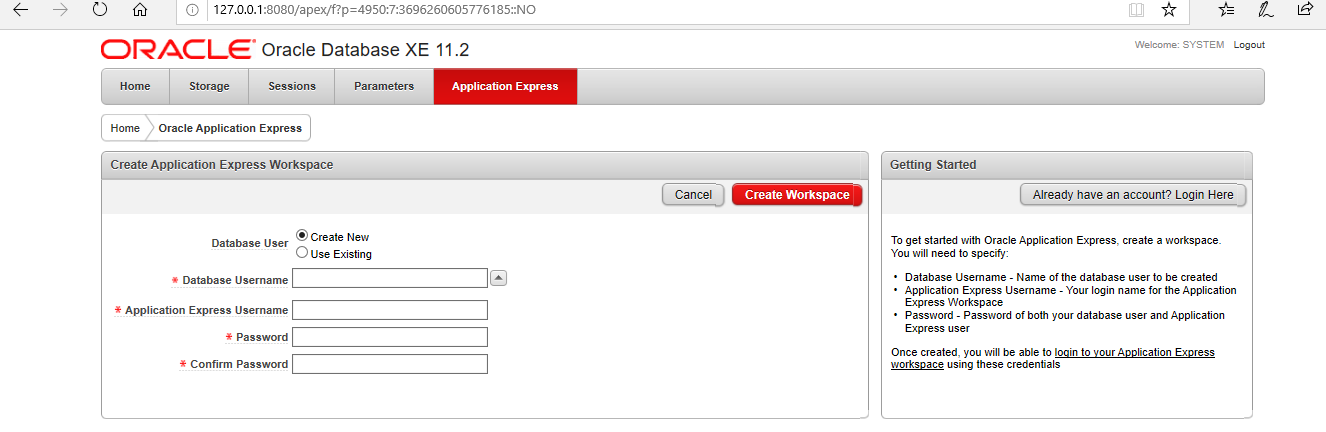
\includegraphics[width=.8\textwidth]{figure/2.PNG}
        \end{center}
    \par Tetapi  jika kamu menggunakan apex online maka search  
    https://apex.oracle.com/en/. Pilih sign in jika kamu sudah memiliki workspace .Masukkan nama database dibuat,nama username dan password tetapi jika kamu belum memiliki akun maka pilih request workspace.Lalu  ikuti langkah-langkah pada  form pendaftaran .Ketika sudah selesai masukkan database,username dan password yang telah dibuat.Jika sudah kamu bisa menggunakan aplikasi tersebut.
    \begin{center}
              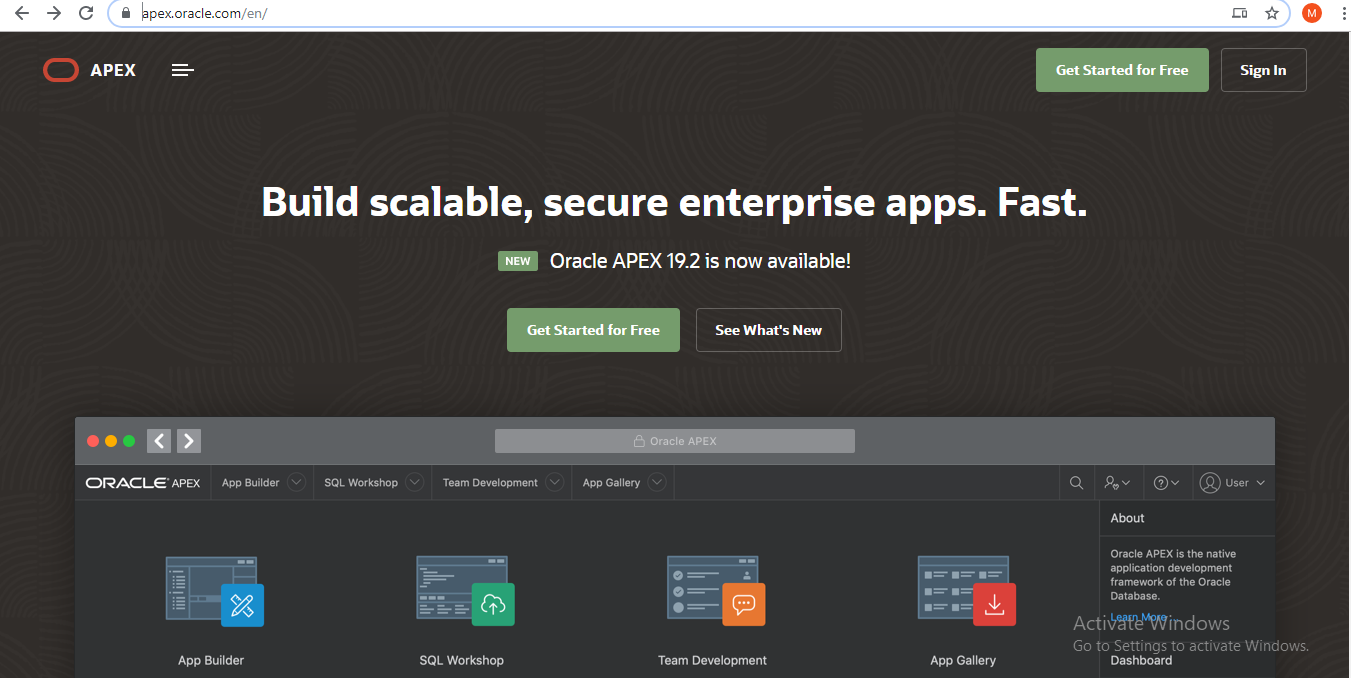
\includegraphics[width=.8\textwidth]{figure/3.PNG}
                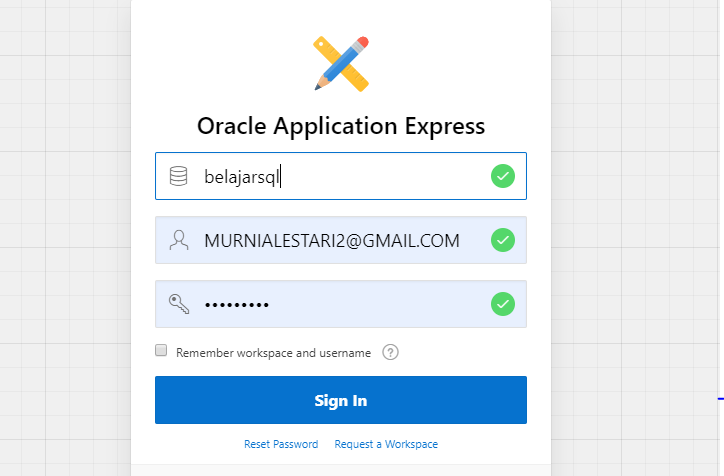
\includegraphics[width=.8\textwidth]{figure/4.PNG}
        \end{center}
    \item Jika kamu sudah menginstall aplikasi oracle apex atau sudah mendaftar di oracle apex online dan setelah itu kalian akan masuk ke dalam aplikasi oracle apex.
    \item Pilih sql workshop dan pilih sql command. Sql command digunakan untuk mengetikkan query yang akan digunakan.
    \item Langkah selanjutnya adalah pembuatan database yang dimulai dnegan membuat table. Disini saya membuat aplikasi hasil pangan yang terdapat enam tabel yaitu kecamatan, kelurahan,komoditas,tanaman,lahan,panen. Query yang diinputkan di sql command seperti berikut :
    \begin{enumerate}
        \item Table kecamatan
        \par Table kecamatan mempunyai 2 kolom yaitu kode kecamatan dan nama kecamatan. Pada table ini yang menjadi primary keynya adalah kode kecamatan.
        \begin{center}
           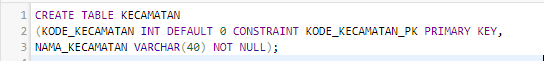
\includegraphics[width=.8\textwidth]{figure/7.PNG} 
        \end{center}
        \item Table kelurahan
        \par Table kelurahan mempunyai 3 kolom yaitu kode kecamatan,kode kelurahan,dan nama kelurahan. Pada table ini kode kecamatan  foreign key dari table kecamatan, dan kode kelurahan merupakan primary key dari table kelurahan.
        \begin{center}
              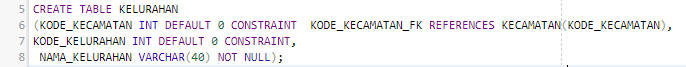
\includegraphics[width=.8\textwidth]{figure/8.PNG}
        \end{center}
        \item Table komoditas
        \par Table komoditas mempunyai 2 kolom yaitu kode komoditas dan jenis komoditas. Pada table  ini kode komoditas dijadikan sebagai primary key.
        \begin{center}
              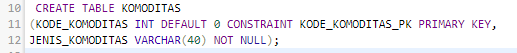
\includegraphics[width=.8\textwidth]{figure/9.PNG}
        \end{center}
        \item Table tanaman
        \par Table tanaman mempunyai empat kolom yaitu kode komoditas,kode tanaman, nama tanaman dan panen ke. Pada  table ini kode komoditas dijadikan sebagai  foreign key dan k ode tanaman merupakan primary key dari table tanaman.
        \begin{center}
              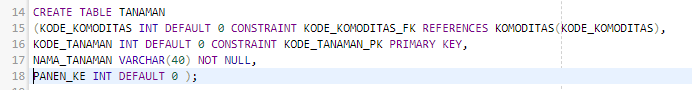
\includegraphics[width=.8\textwidth]{figure/10.PNG}
        \end{center}
        \newpage\item Table lahan
        \par Table lahan mempunyai sembilan kolom yaitu kodel ahan,kode kecamatan,kode tanaman,tahun,bulan,luas lahan sawah,luas non sawah,nama pemilik,alamat pemilik. Pada table ini kode kecamatan dan kode tanaman merupakan foreign key dari table kecamatan dan tanaman. Kode lahan pada table ini dijadikan sebagai primary key.
        \begin{center}
              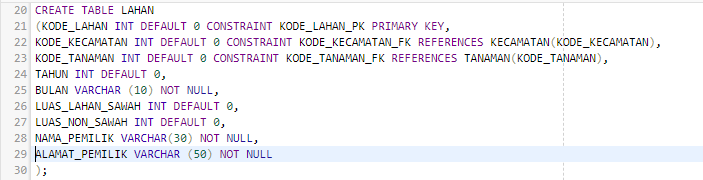
\includegraphics[width=.8\textwidth]{figure/11.PNG}
        \end{center}
        \item Table panen
        \par Table panen mempunyai Sembilan kolom yaitu kode hasil panen,tahun,bulan,kode kelurahan,kode kecamatan,kode tanaman,kode komoditas,kode lahan dan hasil panen. Pada table ini kode kelurahan,kode kecamatan,kode tanaman,kode komoditas,dank ode lahan merupakan foreign key dari table kecamatan,kelurahan,tanaman,komoditas,dan lahan. Kode hasil panen pada table ini merupakan primary key.
        \begin{center}
              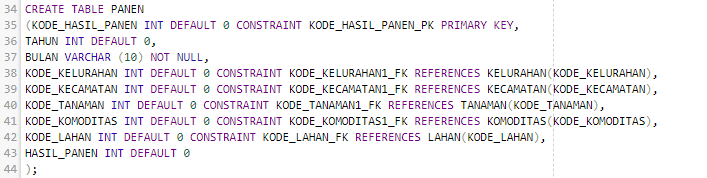
\includegraphics[width=.8\textwidth]{figure/12.PNG}
        \end{center}
    \end{enumerate}
    \item Setelah membuat table maka selanjutnya adalah mengisi baris pada kolom table yang telah dibuat. Berikut adalah cara menambahkan baris pada kolom :
    \begin{enumerate}
        \item Table kecamatan
        \par Pada table kecamatan mempunyai  dua kolom maka baris yang dimasukkan juga sebanyak dua baris sesuai dengan jumlah kolom.
         \begin{center}
              
\includegraphics[width=.8\textwidth]{figure/13.PNG}
        \end{center}
        \newpage\item Table kelurahan
        \par Pada table kelurahan mempunyai tiga kolom maka baris yang dimasukkan juga sebanyak tiga baris sesuai dengan jumlah kolom, akan tetapi pada kode kecamatan kita masukkan kode kecamatan yang sudah kita buat sebelumnya pada table kecamatan karena kode kecamatan merupakan foreign key  yang diambil dari table kecamatan.
         \begin{center}
              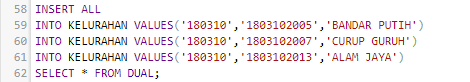
\includegraphics[width=.8\textwidth]{figure/14.PNG}
        \end{center}
        \item Table komoditas
        \par Pada table komoditas mempunyai dua kolom maka baris yang dimasukkan juga dua baris sesuai dengan jumlah kolom yang dibuat.
         \begin{center}
              
\includegraphics[width=.8\textwidth]{figure/15.PNG}
        \end{center}
        \item Table tanaman
        \par Pada table tanaman mempunyai tiga kolom maka baris yang akan dimasukkan juga tiga baris sesuai dengan jumlah kolom yang dibuat,akan tetapi kode komoditas merupakan foreign key yang diambil dari table komoditas sehingga isikan baris sesuai yang dibuat pada table komoditas.
         \begin{center}
              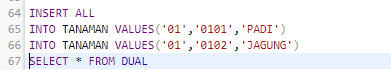
\includegraphics[width=.8\textwidth]{figure/16.PNG}
        \end{center}
         \item Table lahan
        \par Pada table lahan mempunyai sepuluh kolom maka baris yang akan dimasukkan juga sebnayak sepuluh baris sesuai dengan jumlah kolom,akan tetapi perhatikan foreign key yang diambil dari table kelurahan,kecamatan dan juga tanaman harus sesuai dengan yang sudah dimasukkan dalam table sebelumnya.
         \begin{center}
              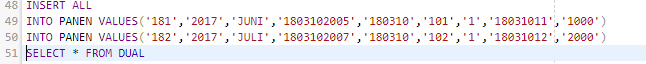
\includegraphics[width=.8\textwidth]{figure/17.PNG}
        \end{center}
        \newpage\item Table panen
        \par Pada table panen mempunyai mempunyai sembilan kolom maka baris yang dimasukkan juga sebanyak Sembilan baris sesuai dengan kolom pada table tersebut,akan tetapi jangan lupa pada table panen terdapat foreign key dari table kecamatan,kelurahan,tanaman,komoditas,serta lahan maka masukkan isi baris sesuai dengan  isi baris yang telah dimasukkan pada table selanjutnya.
         \begin{center}
              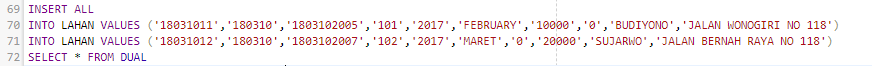
\includegraphics[width=.8\textwidth]{figure/18.PNG}
        \end{center}
    \end{enumerate}
    \item Setelah column dan baris diisi maka selanjutnya adalah pembuatan  fungsi trigger. Fungsi trigger adalah fungsi yang digunakan untuk menampilkan suatu data secara otomatis pada saat insert,delete dan update pada table. Berikut merupakan trigger yang dibuat :
    \begin{center}
              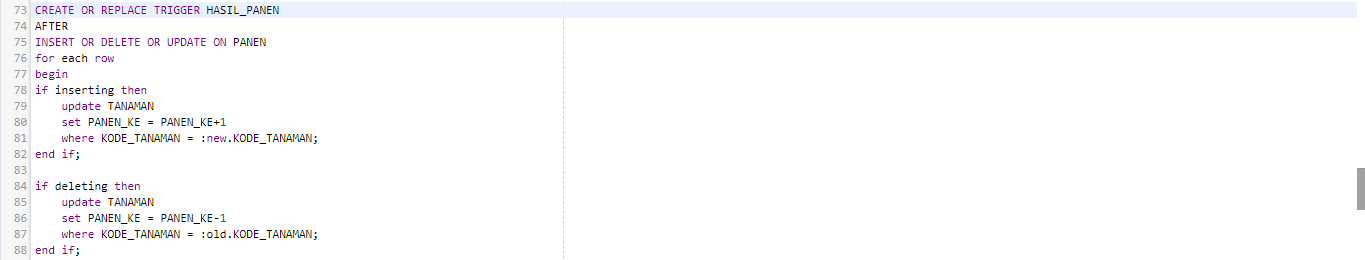
\includegraphics[width=.8\textwidth]{figure/19.PNG}
        \end{center}
        \begin{center}
              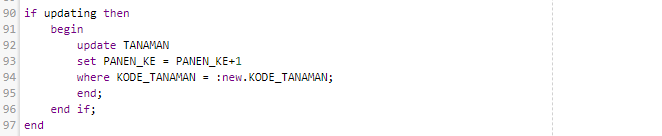
\includegraphics[width=.8\textwidth]{figure/20.PNG}
        \end{center}
        \par Pada aplikasi ini saya membuat  trigger yang bernama HASIL PANEN, yang mana ketika kita menginsert,mendelete dan mengupdate pada table PANEN maka yang akan mengalami perubahan secara otomatis pada table TANAMAN  tepatnya di colum PANEN KE.
        \item Setelah itu adalah tahapan membuat view pada aplikasi. View merupakan perintah untuk menggabungkan query join,innerjoin  table dengan lebih sederhana.
        \begin{center}
              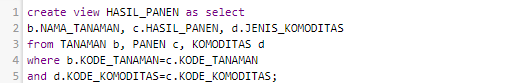
\includegraphics[width=.8\textwidth]{figure/21.PNG}
        \end{center}
        \par Jadi contoh pada view tersebut akan menampilkan nama tanaman,hasil panen, jenis komoditas dimana nama tanaman,hasil panen,dan jenis komoditas pada table yang berbeda. Jadi view lebih menyederhanakan query yang dimasukkan.
        \item Selanjutnya adalah pembuatan sinonim. Sinonim  digunakan untuk memanggil nama table dengan nama yang berbeda.
        \begin{center}
              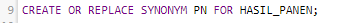
\includegraphics[width=.8\textwidth]{figure/22.PNG}
        \end{center}
        \par Contohnya table HASIL PANEN dapat dipanggil dengan nama PN.
        \item Setelah  semuanya selesai ,maka selanjutnya adalah pembuatan aplikasi dengan memilih  app builder.
        \begin{center}
              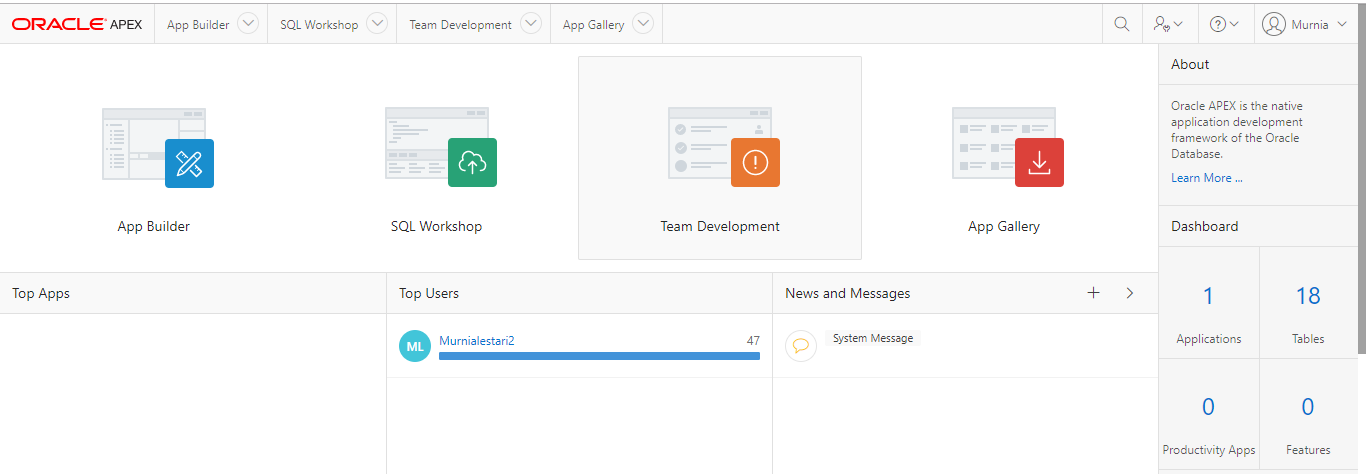
\includegraphics[width=.8\textwidth]{figure/23.PNG}
        \end{center}
        \item setelah itu pilih create untuk membuat aplikasi yang baru dengan menggunakan data-data yang telah dibuat di oracle apex.
        \begin{center}
              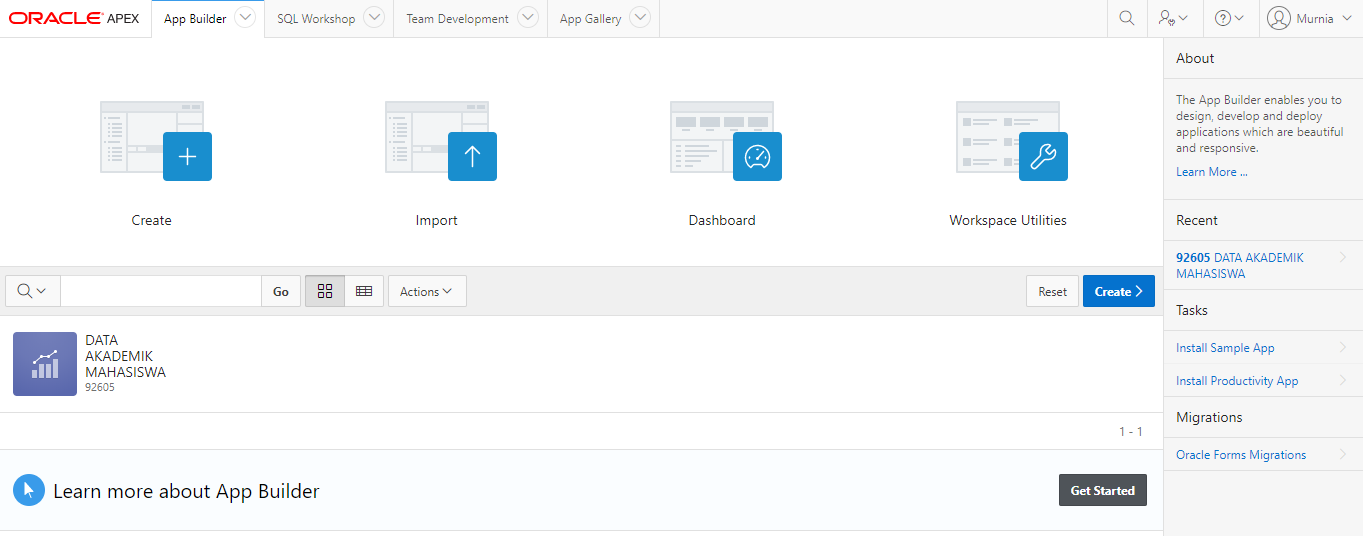
\includegraphics[width=.8\textwidth]{figure/24.PNG}
        \end{center}
        \item Selanjutnya pilih new application yang digunakan untuk membuat aplikasi.
        \begin{center}
              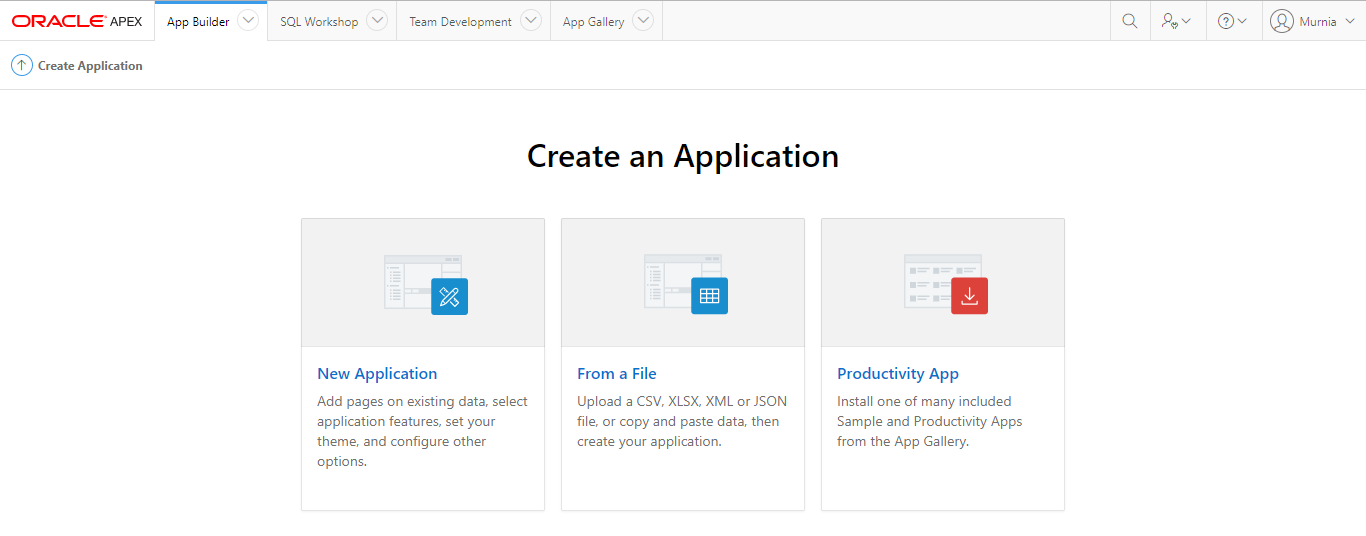
\includegraphics[width=.8\textwidth]{figure/25.PNG}
        \end{center}
        \item Buatlah nama aplikasi yang akan dibuat,lalu pilih add page untuk memilih page yang akan digunakan untuk membuat aplikasi.
        \begin{center}
              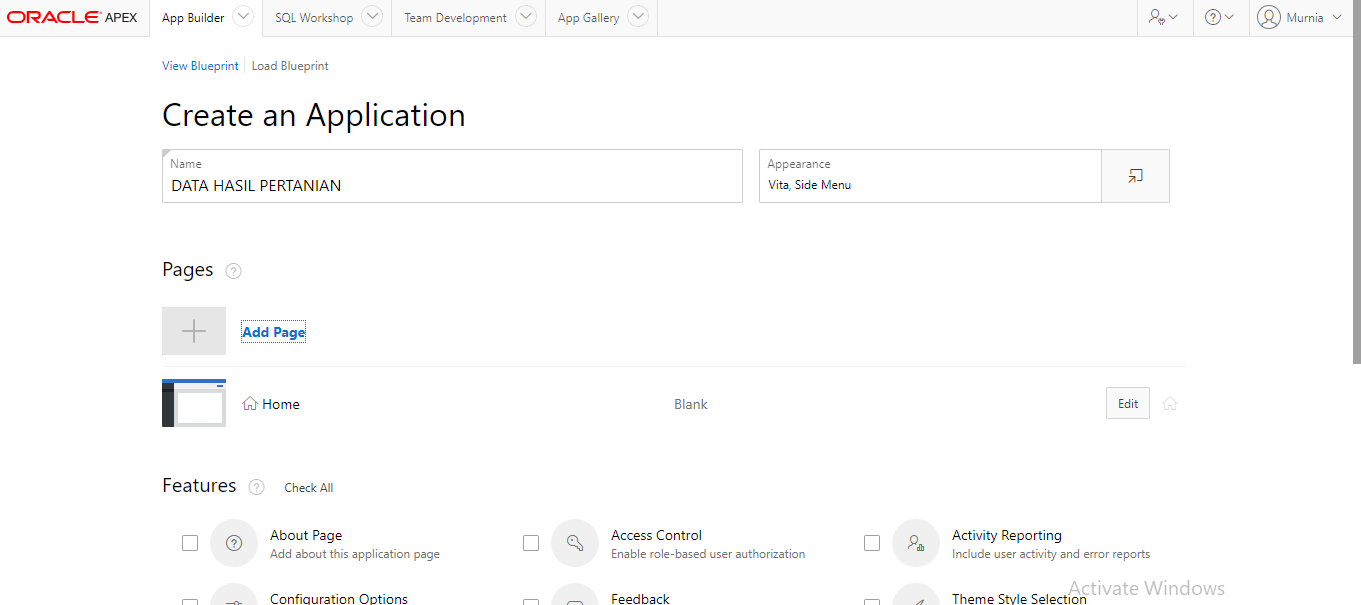
\includegraphics[width=.8\textwidth]{figure/26.PNG}
        \end{center}
        \item Pilih interactive report untuk page aplikasi yang dibuat.
         \begin{center}
              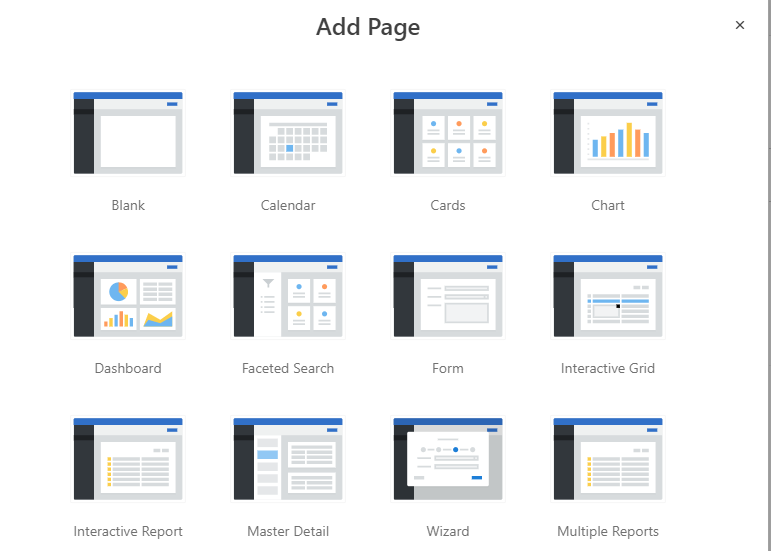
\includegraphics[width=.8\textwidth]{figure/27.PNG}
        \end{center}
        \newpage\item Setelah itu  isi page namenya dengan kecamatan yang merupakan table pertama pada aplikasi. Pilih table kecamatan pada table or view lalu add page.
        \begin{center}
              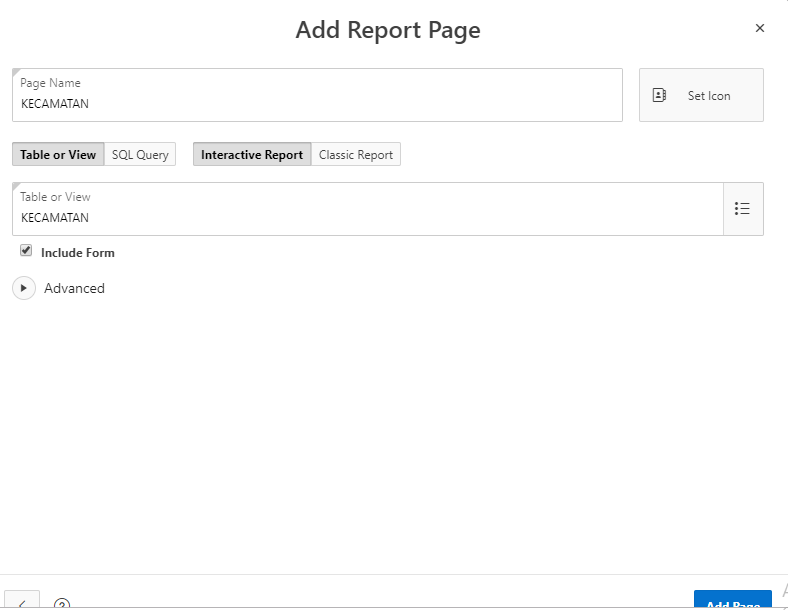
\includegraphics[width=.8\textwidth]{figure/28.PNG}
        \end{center}
        \item Lakukan hal yang sama pilih add page dan pilih page intercative report lalu isi name page dengan kelurahan,komoditas,tanaman,lahan dan panen secara bergantian. Lalu pilih table atau view table yang yang telah dibuat yaitu kelurahan,komoditas,tanaman,lahan,dan panen juga secara bergantian. Jangan lupa jika ingin menambahkan view yang telah dibuat dengan nama hasil panen pada page name lalu pilih view yang telah dibuat yaitu hasil panen. Lalu add page.
        \begin{center}
              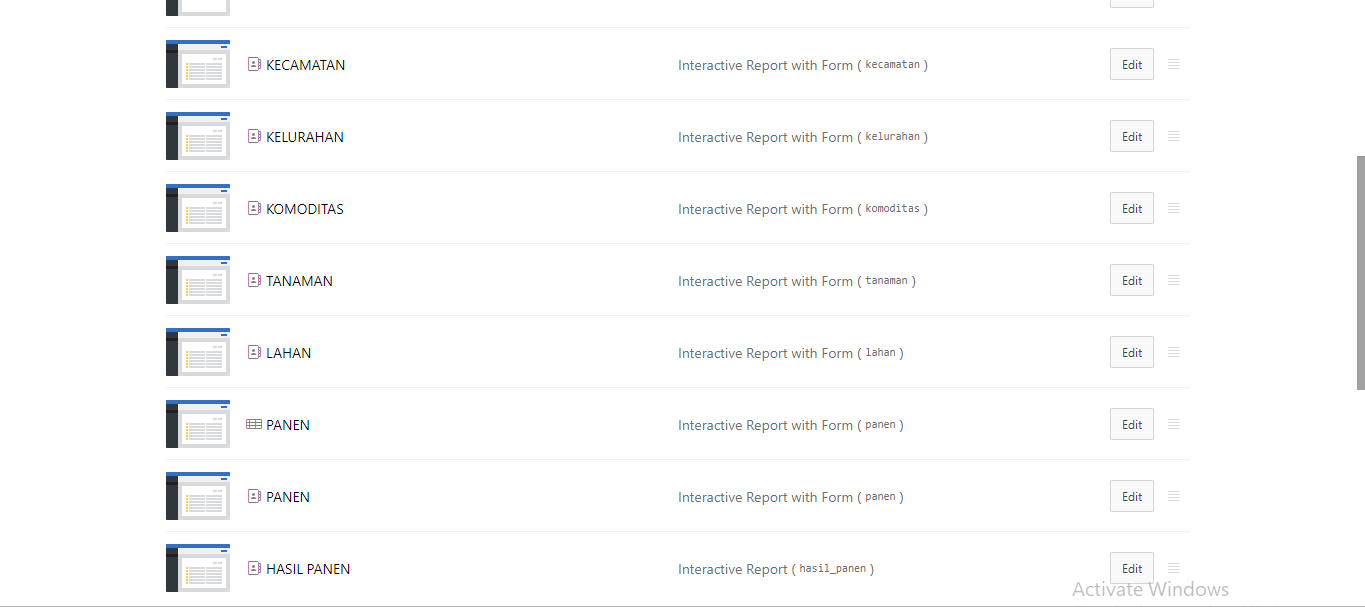
\includegraphics[width=.8\textwidth]{figure/29.PNG}
        \end{center}
       \newpage \item Setelah semuanya di add page maka pada features di cek all. Maka setelah itu create application. Tungga hingga selesai.
        \begin{center}
              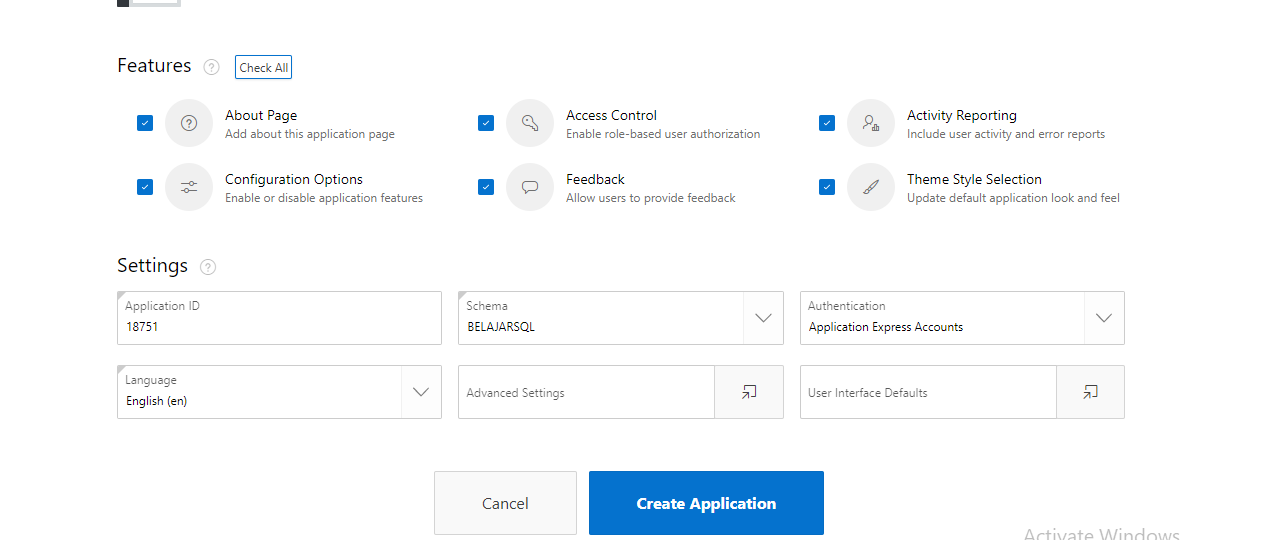
\includegraphics[width=.8\textwidth]{figure/30.PNG}
        \end{center}
         \item Setelah itu pilih run application untuk melihat aplikasi yang sudah dibuat.
         \begin{center}
              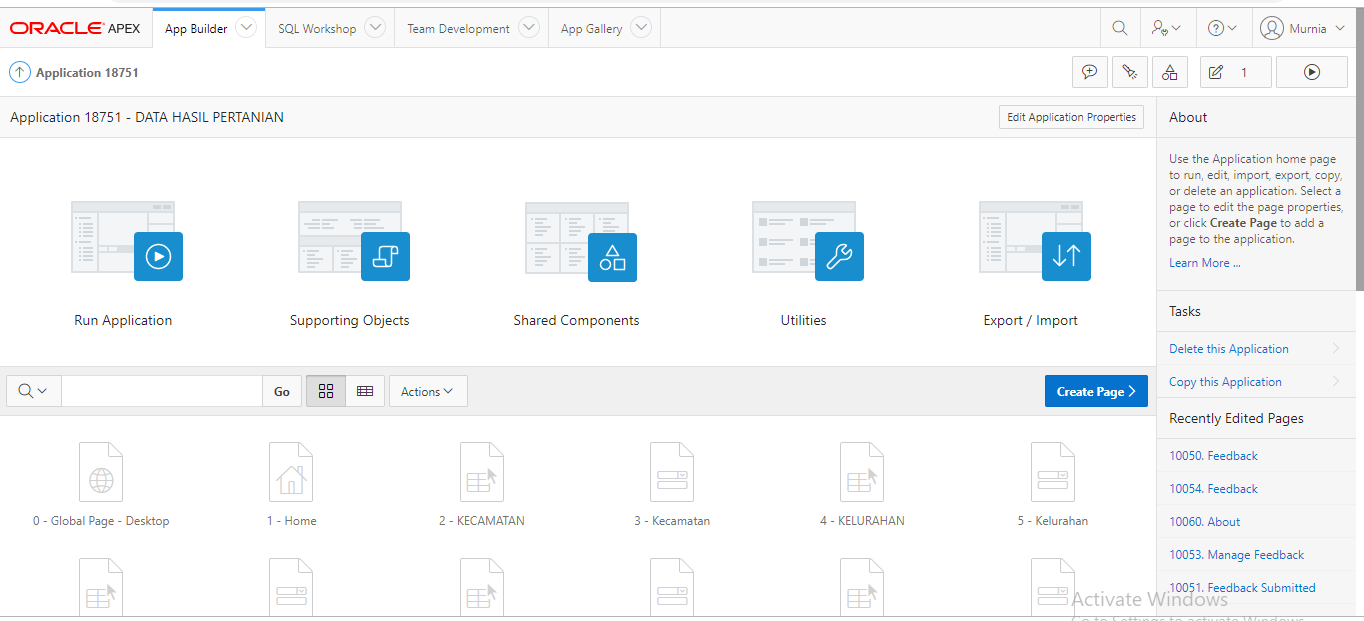
\includegraphics[width=.8\textwidth]{figure/31.PNG}
        \end{center}
        \item Dan masukkan username dan password untuk melihat aplikasi yang telah dibuat. Lalu sign in.
        \begin{center}
              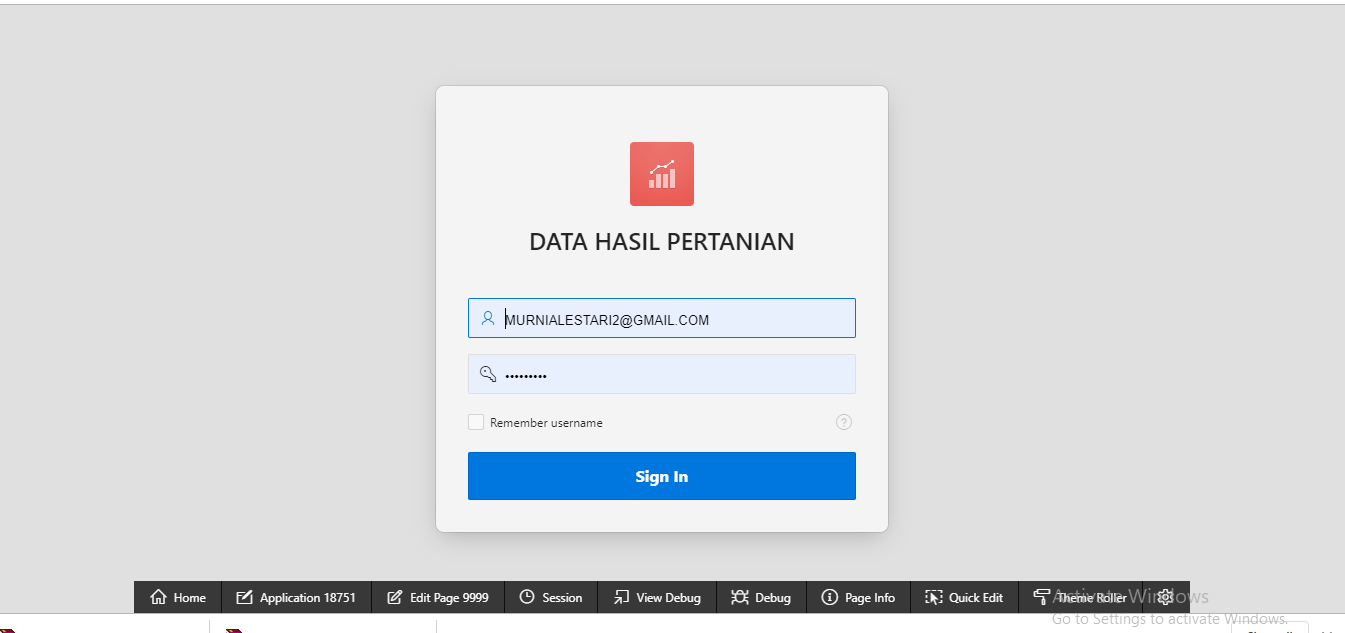
\includegraphics[width=.8\textwidth]{figure/32.PNG}
        \end{center}
        \newpage\item Maka aplikasi data hasil pertanian sudah selesai dibuat. 
        \begin{center}
              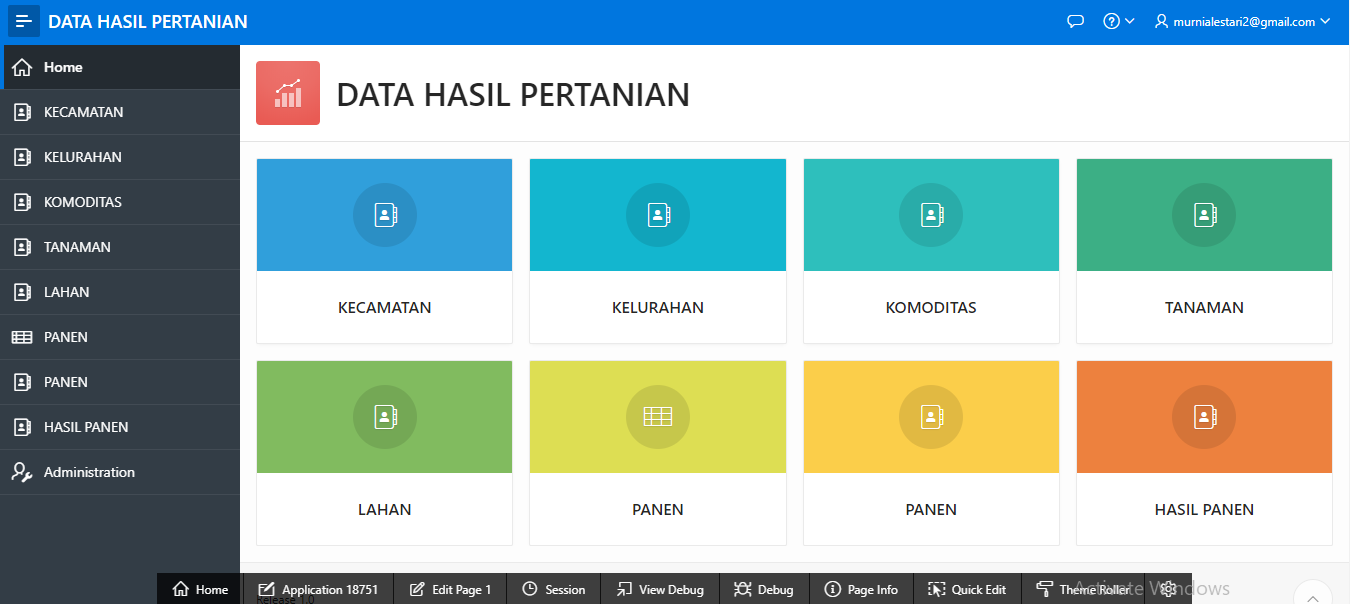
\includegraphics[width=.8\textwidth]{figure/33.PNG}
        \end{center}
\end{enumerate}
\usepackage{listings} https://apex.oracle.com/pls/apex/f?p=18751:LOGIN_DESKTOP:703118311964605:::::
\par User Name : MURNIALESTARI2@GMAIL.COM
PASSWORD : murnia123
\end{document}
